\section{Docker}
\begin{frame}
  \vfill
  ¿Qué es Docker?
  \vfill
\end{frame}

\begin{frame}{¿Qué es Docker?}
  \begin{itemize}[<+->]
    \item Docker permite empaquetar y ejecutar una aplicación en containers aislados.
    \item Docker Engine está dividido en 3 componentes: el demonio
      \textbf{dockerd}, una \textbf{API REST} y la CLI \textbf{docker}.
    \item Usos posibles:
      \begin{itemize}[<+->]
        \item En desarrollo/Testing.
        \item Escalado y despliegue (deployment).
        \item Más servicios en un equipo sin VMs.
      \end{itemize}
  \end{itemize}
\end{frame}


\begin{frame}{¿Cómo funciona?}
  Docker es una herramienta que utiliza una serie de características del kernel
  para proveer containers:
  \begin{description}[<+->]
    \item[Namespaces:] Docker lo utiliza para proveer el espacio de trabajo
      aislado que denominamos container. Por cada container Docker crea un
      conjunto de espacios de nombres (entre ellos \textbf{pid}, \textbf{net},
      \textbf{ipc} y \textbf{mnt}).
    \item[Control groups:] Para, opcionalmente, limitar los recursos asignados
      a un contenedor.
    \item[Union file systems:] Se utilizan como filesystem de los containers.
        Docker puede utilizar \textbf{overlay2}, \textbf{AUFS},
        \textbf{btrfs}, \textbf{vfs} y \textbf{DeviceMapper}.
  \end{description}
\end{frame}

\begin{frame}{Containers VS VMs}
    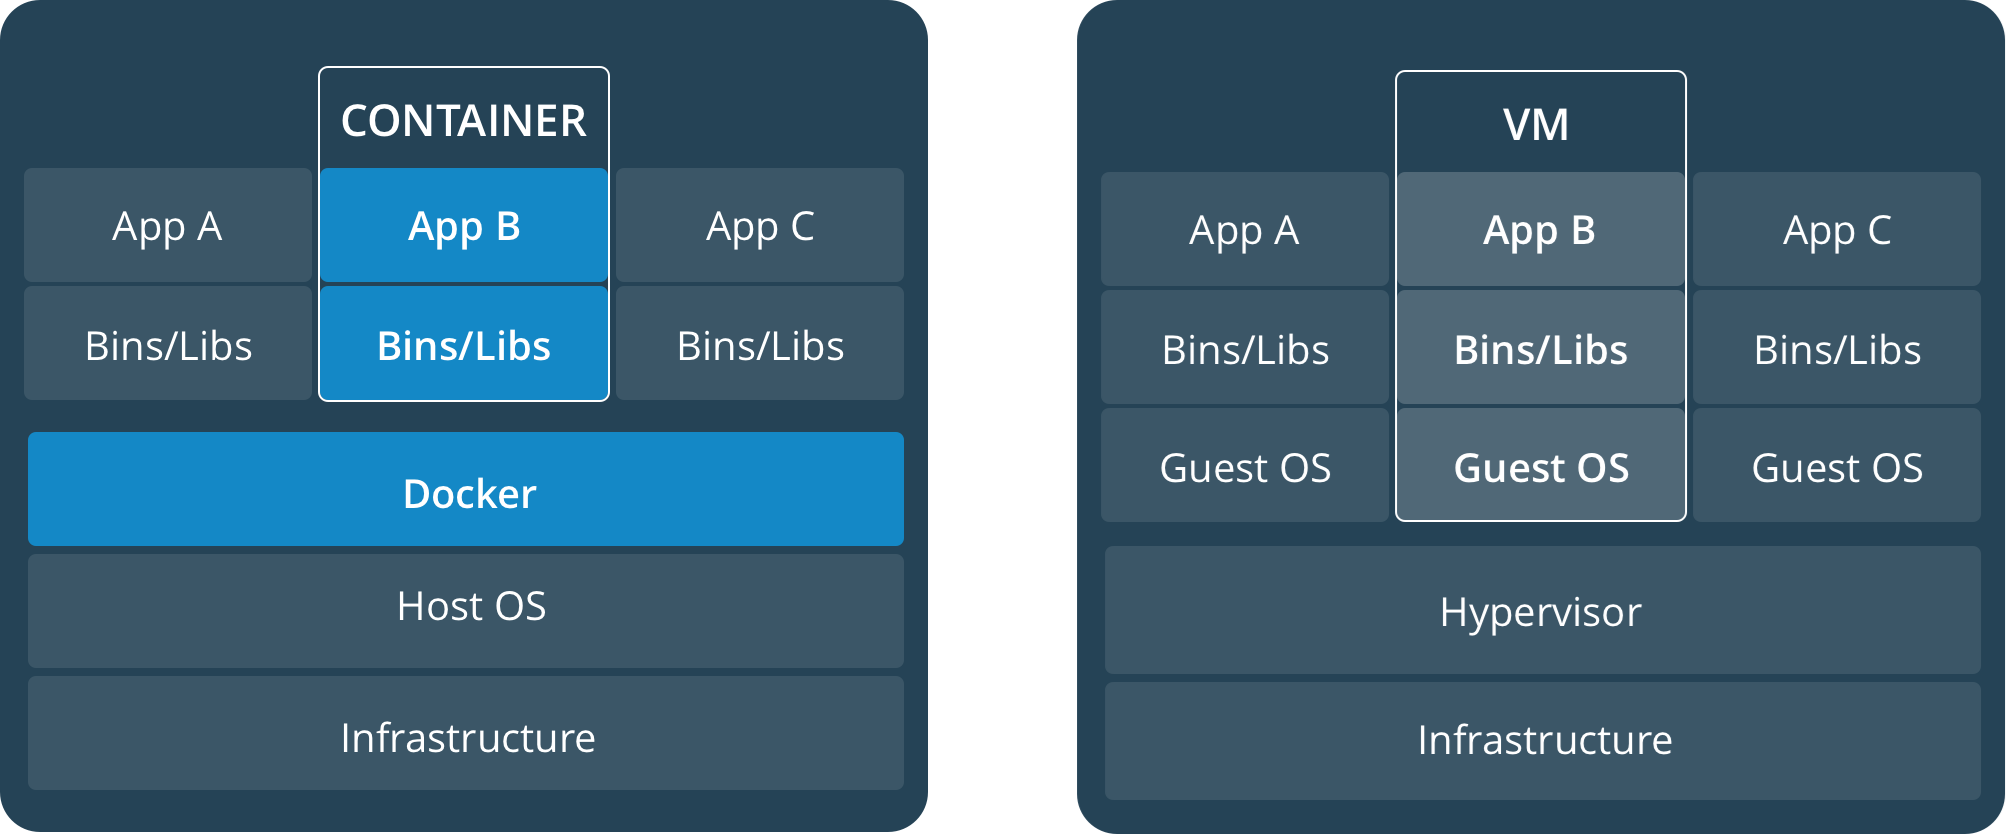
\includegraphics[width=\linewidth]{imagenes/containervsvm}
    \footnote{\url{https://docs.docker.com/get-started/\#containers-and-virtual-machines}}
\end{frame}

\begin{frame}{Definiciones}
    \begin{description}[<+->]
        \item[imagen:] Paquete (sólo lectura) que contiene todo lo necesario
            para ejecutar una aplicación (librerías, configuraciones, etc...).
        \item[registry:] Es un almacén de imágenes de Docker, por defecto
            docker utiliza \textit{Docker Hub}.
        \item[container:] Es una instancia de una imagen en ejecución.
        \item[Dockerfile:] Archivo que define como construir una imagen.
    \end{description}
    Una imagen puede basarse en otras, por ejemplo:
    \textbf{httpd~\textrightarrow~debian:jessie-backports~\textrightarrow~debian:jessie~\textrightarrow~scratch}
    donde \textit{scratch} es un nombre especial que significa
    que se inicia desde una imagen vacía.
\end{frame}

\begin{frame}[fragile]{Comandos básicos}
    \begin{lstlisting}[language=bash,basicstyle=\normalsize]
# Descargar imagen de Apache de DockerHUB
docker pull httpd
# Ejecutar imagen
docker run httpd
# Crear una imagen a partir de un Dockerfile
docker image build -t NOMBRE_TAG .
# Ejecutar la imagen creada
docker run NOMBRE_TAG
# Subir la imagen a DockerHUB
# antes hay que ejecutar `docker login`
docker push NOMBRE_TAG\
        USUARIO_DOCKERHUB/REPOSITORIO
    \end{lstlisting}
\end{frame}

\begin{frame}{Arquitectura}
    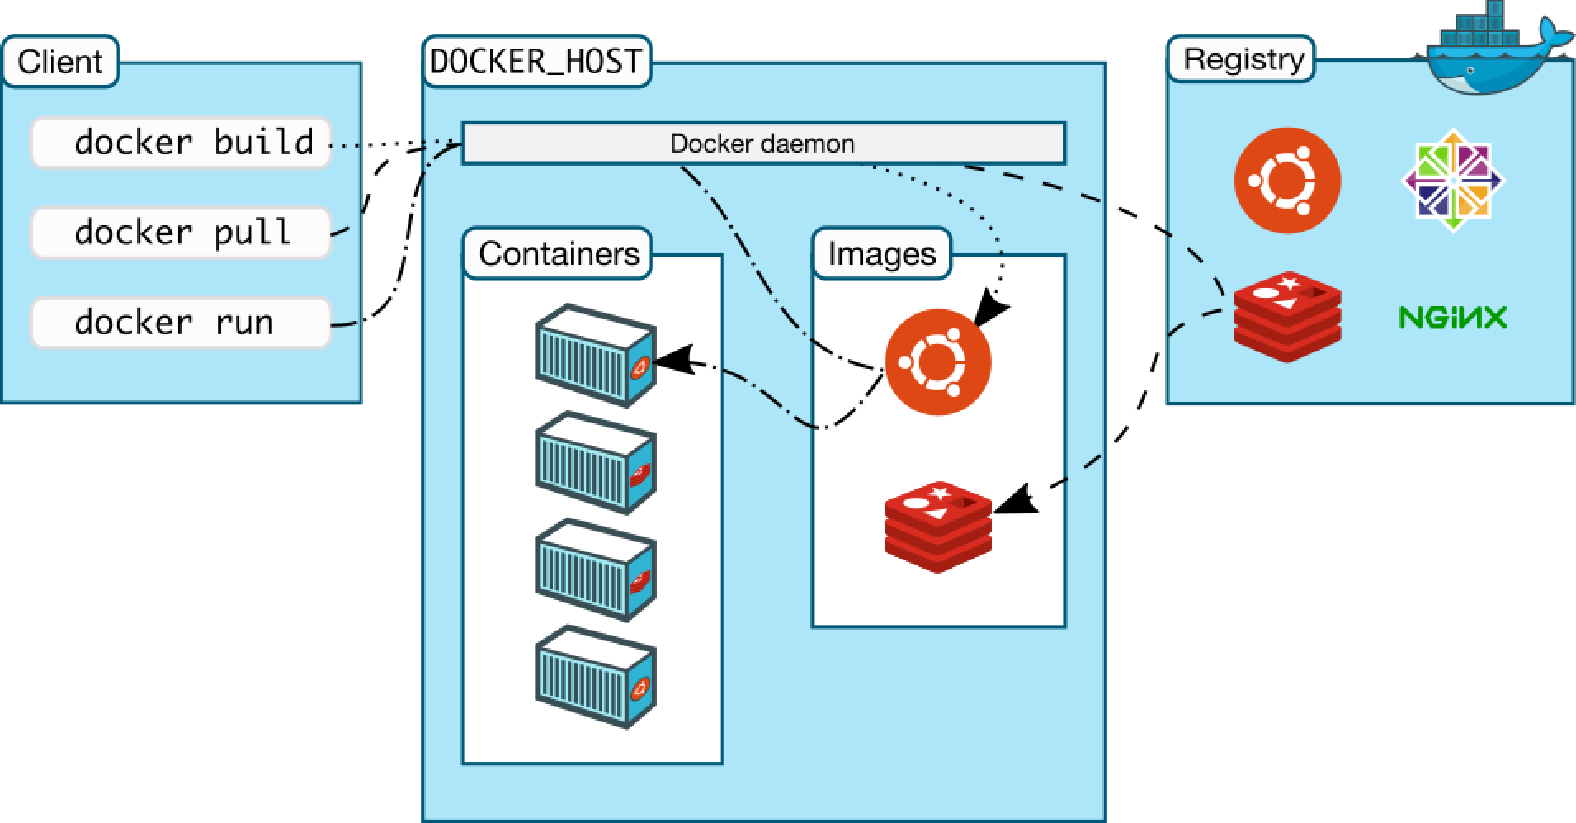
\includegraphics[width=\linewidth]{imagenes/architecture}
    \footnote{\url{https://docs.docker.com/engine/docker-overview/\#docker-architecture}}
\end{frame}

\begin{frame}[fragile]{Comandos básicos}
    \begin{lstlisting}[language=bash,basicstyle=\normalsize]
# Información general y configuración
docker info
# Containers en ejecución
docker ps
# Imágenes y containers
docker image ls
docker container ls -a
# Ejecutar el container de Ubuntu en modo interactivo (bash)
docker pull ubuntu &&\
    docker run -v ./dir_comp:/mnt -it ubuntu
# Crear una nueva imagen con los cambios del container
docker commit CONTAINER REPOSITORY:TAG
    \end{lstlisting}
\end{frame}

\begin{frame}{Capas}
    \begin{itemize}[<+->]
            \item Cada imagen está compuesta de una serie de capas.
            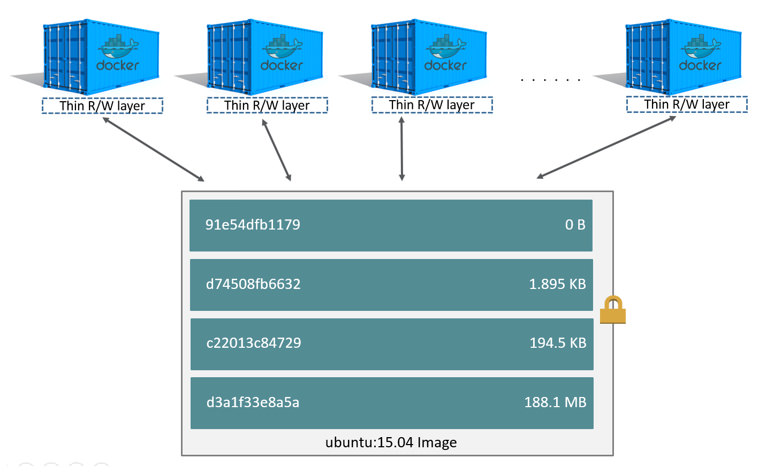
\includegraphics[width=0.6\linewidth]{imagenes/sharing-layers}
            \item Las capas se montan una sobre otra.
            \item Solo la última es R/W (la capa del container)
    \end{itemize}
    \footnote{\url{https://docs.docker.com/storage/storagedriver/\#container-and-layers}}
\end{frame}

\begin{frame}{Referencias}
  \begin{itemize}
    \item \url{https://docs.docker.com/engine/docker-overview/\#docker-objects}
    \item \url{https://docs.docker.com/engine/reference/commandline/}
    \item \url{https://medium.com/@nagarwal/understanding-the-docker-internals-7ccb052ce9fe}
    \item \url{http://docker-saigon.github.io/post/Docker-Internals/}
    \item \url{https://www.safaribooksonline.com/library/view/using-docker/9781491915752/}
    \item \url{https://washraf.gitbooks.io/the-docker-ecosystem}
  \end{itemize}
\end{frame}



